\documentclass{scrartcl}

\usepackage[utf8]{inputenc}
\usepackage{tikz}
\usepackage{url}
\usepackage{mdframed}
\usepackage{listing}

\usepackage{hyperref}

\usetikzlibrary{decorations.pathreplacing, angles, quotes, matrix}

\newcommand{\tushan}{\textsc{Tushan}}

\begin{document}
This document is the specification of \tushan{}. It contains the 
definitions of game rules, logical entities and their representation and 
protocol specification.

\section{Game Description}
\tushan{} is based on the game 
\href{https://en.wikipedia.org/wiki/Ta\_Y\%C3\%BC}{Ta-Yü}. Two players
oppose each other on a quadratic field which is separated in cells. Each player 
is assigned two opposite sites of the field. In turns the player place stones
which cover cells. The stones are equipped with connectors on its sites. These
connectors form a flow through the stones. The game ends if there are no valid
placements of the current stone and every player is awarded the product of two
factors, where each factor corresponds to the number of connectors immediately
touching the sites of the field (of said player). These notions are specified
in the following.

\section{Entities}
\subsection{Field}
The field of the game.
\subsubsection{Description}
The field is a quadratic collection of cells. Each cell is identified by its 
coordinates starting with $(0,0)$ at the top left and proceeding to the left 
with increasing first element and to the bottom with increasing second element.
\subsubsection{Illustration}
\begin{mdframed}
  \begin{center}
    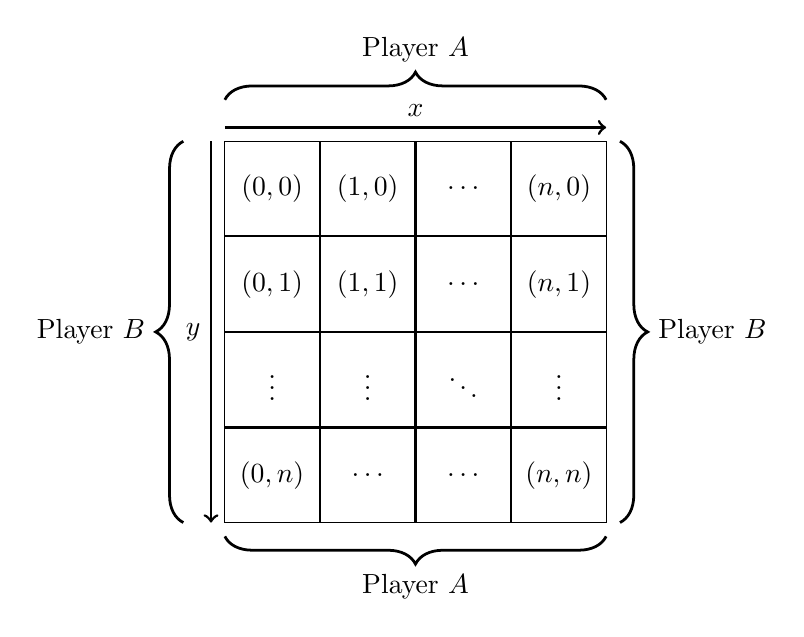
\begin{tikzpicture}
      \matrix (field) [
        matrix of nodes,
        column sep = 0pt,
        row sep = 0pt,
        nodes in empty cells,
        inner xsep = 0pt,
        nodes = {
          rectangle, draw, minimum width = 1.2cm, minimum height = 1.2cm, 
          outer sep = 0pt, inner xsep = 0pt, inner ysep = 0pt, anchor = center
        }] {
          $(0,0) $ & $(1,0) $ & $\dots $ & $(n,0) $ \\
          $(0,1) $ & $(1,1) $ & $\dots $ & $(n,1) $ \\
          $\vdots$ & $\vdots$ & $\ddots$ & $\vdots$ \\
          $(0,n) $ & $\dots $ & $\dots $ & $(n,n) $ \\
      };
      \draw [ decoration = { brace, raise = 15pt, amplitude = 10pt }, decorate, 
        line width = 1pt ]
          (field-1-1.north west) -- node [above, yshift = 25pt] {Player $A$} 
          (field-1-4.north east);
      \draw [ decoration = { brace, raise = 5pt, amplitude = 10pt, mirror }, 
        decorate, line width = 1pt ]
          (field-4-1.south west) -- node [below, yshift = -15pt] {Player $A$} 
          (field-4-4.south east);
      \draw [ draw, -> , line width = 1pt] ([yshift = 5pt] field-1-1.north west) 
        to node [above] {$x$} ([yshift = 5pt] field-1-4.north east);
      \draw [ draw, -> , line width = 1pt] ([xshift = -5pt] field-1-1.north west) 
        to node [left] {$y$} ([xshift = -5pt] field-4-1.south west);
      \draw [ decoration = { brace, raise = 15pt, amplitude = 10pt, mirror }, 
        decorate, line width = 1pt ]
          (field-1-1.north west) -- node [left, xshift = -25pt] {Player $B$} 
          (field-4-1.south west);
      \draw [ decoration = { brace, raise = 5pt, amplitude = 10pt }, 
        decorate, line width = 1pt ]
          (field-1-4.north east) -- node [right, xshift = 15pt] {Player $B$} 
          (field-4-4.south east);
    \end{tikzpicture}
  \end{center}
\end{mdframed}
\subsubsection{Representation}
\end{document}
